\documentclass[10pt, aspectratio=169]{beamer}

% --- Configuración del Tema ---
\usetheme{metropolis}
\usecolortheme{owl} 
\usepackage[spanish]{babel}
\usepackage[utf8]{inputenc}
\usepackage{amsfonts, amsmath, amssymb, amsthm}
\usepackage{graphicx}
\usepackage{tikz}
\usetikzlibrary{decorations.pathmorphing}
\usetikzlibrary{positioning}

% --- Entornos Matemáticos ---
\newtheorem{definicion}{Definición}

% --- Colores Personalizados ---
\definecolor{diagonalred}{RGB}{140, 20, 40}
\definecolor{siliconblue}{RGB}{40, 100, 200}
\definecolor{nhole}{RGB}{200, 50, 50}

\title{La Termodinámica de la Lógica}
\subtitle{Sesión 7: El Cristal, el Ruido y el Transistor}
\author{Rosh Guadiana}
\date{Verano 2026}

\begin{document}

\maketitle

% ==========================================
% ACTO 1: LA ASFIXIA DE LA INFORMACIÓN
% ==========================================

\begin{frame}{El Regreso a la Materia}
    \begin{columns}
        \begin{column}{0.4\textwidth}
            \begin{center}
                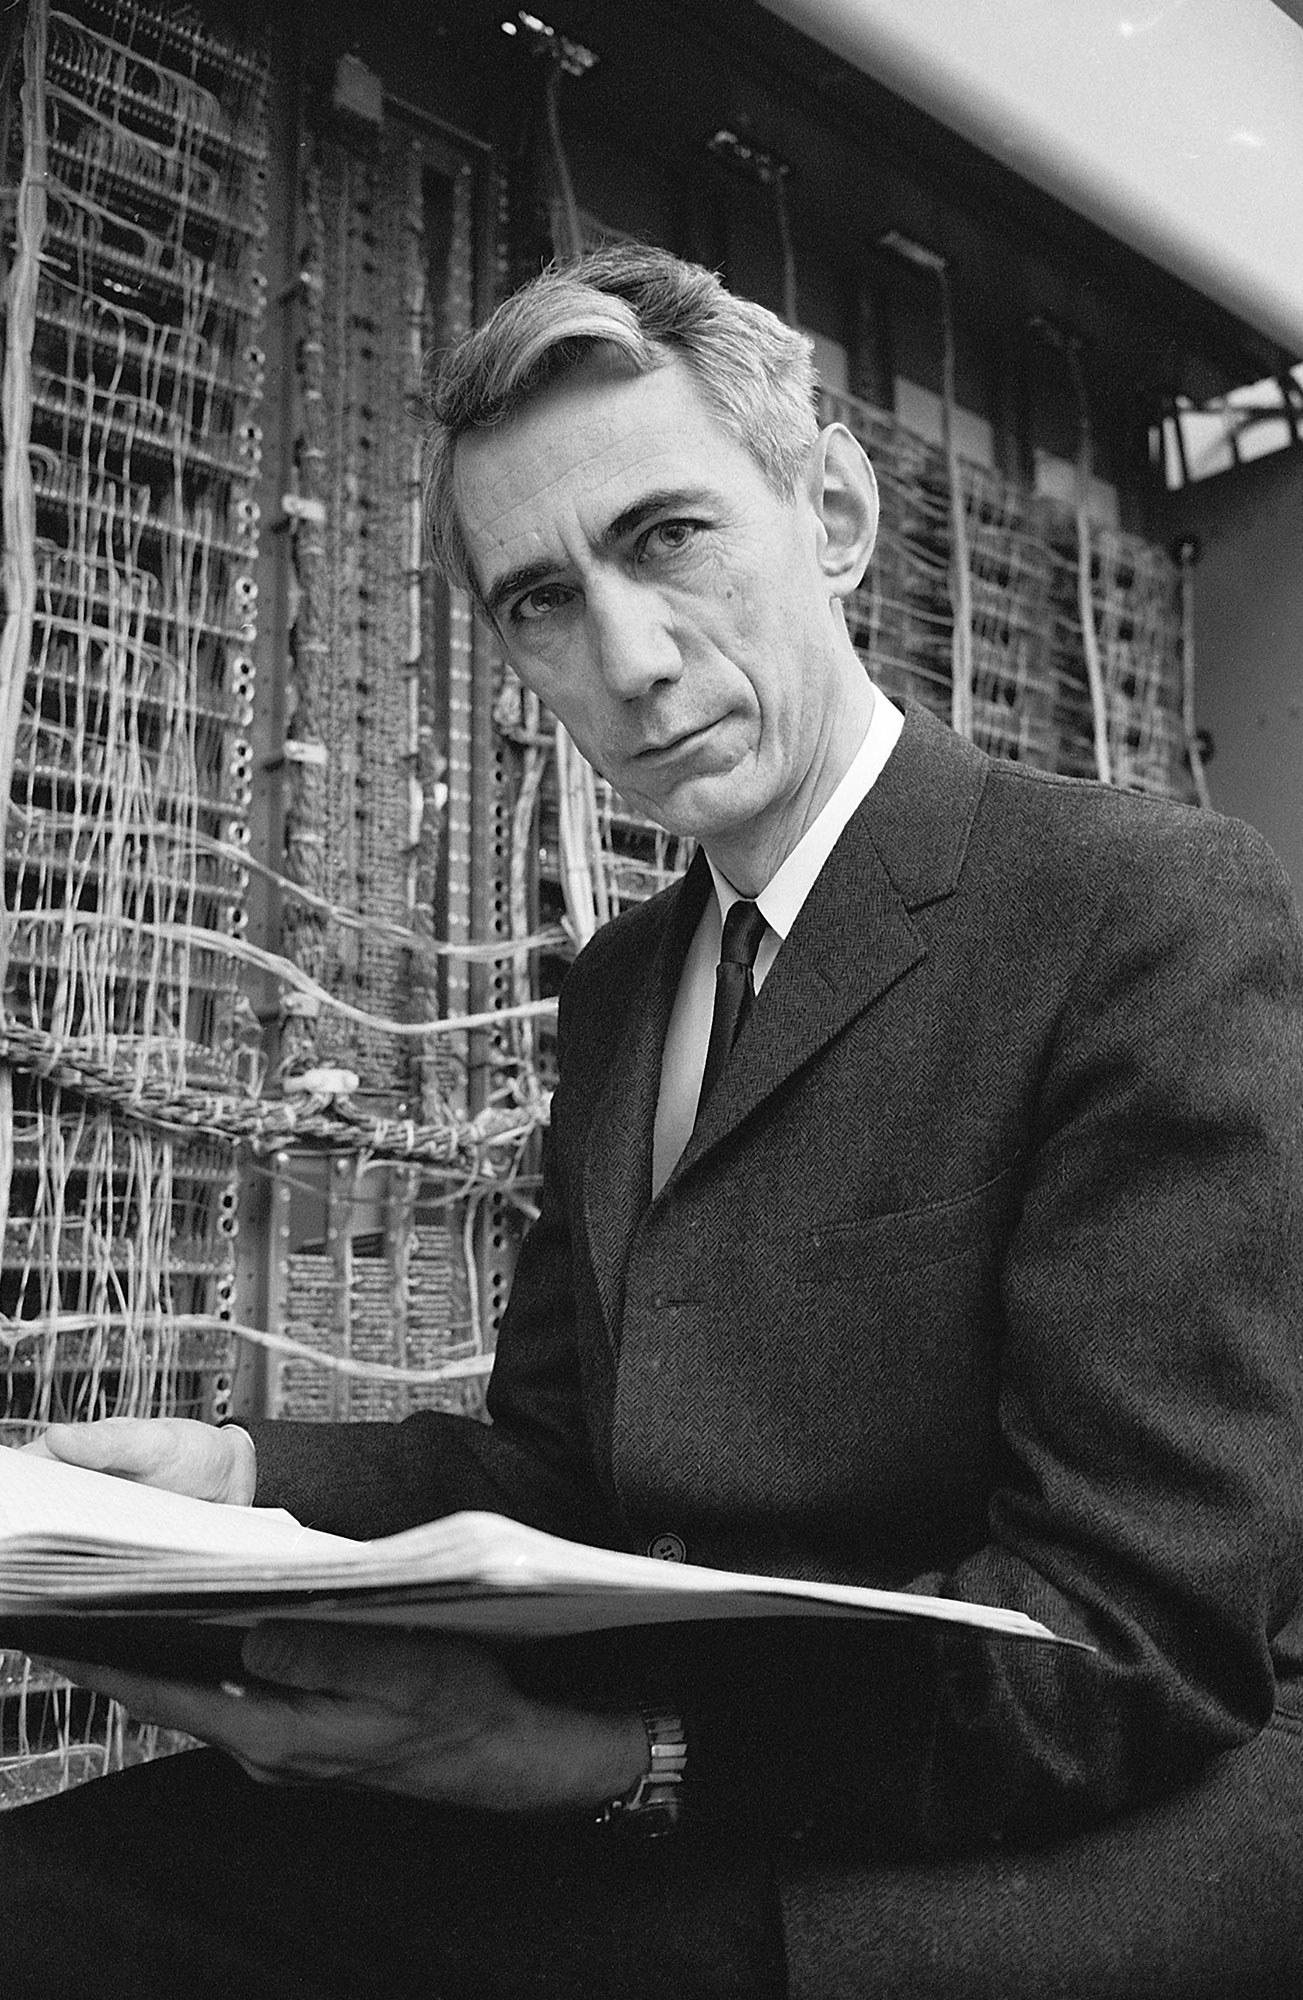
\includegraphics[height=0.65\textheight]{../../assets/Claude-Shannon.jpg} \\
                \vspace{0.2cm}
                \textbf{Claude Shannon} \\
                \small (1916 -- 2001)
            \end{center}
        \end{column}
        \begin{column}{0.6\textwidth}
            \vspace{0.5cm}
            \Large \textbf{El Bit en el Mundo Físico}
            
            \vspace{0.4cm}
            \normalsize
            Hemos establecido que la lógica de Boole puede mapearse en relés e interruptores. 
            
            \vspace{0.4cm}
            Sin embargo, al sacar la sintaxis del vacío matemático y forzarla a existir en la \textbf{materia física}, surge un enemigo inevitable: las leyes de la termodinámica.
        \end{column}
    \end{columns}
\end{frame}

\begin{frame}{El Enemigo Termodinámico}
    \vspace{0.4cm}
    \Large \textbf{El caos del universo contra el orden del bit}
    
    \vspace{0.6cm}
    \normalsize
    Imagina enviar una señal lógica pura (un 1 y un 0) a través de un conductor metálico lineal ordinario, como un cable de cobre.
    
    \vspace{0.4cm}
    El universo no está estático; está lleno de \alert{\textbf{ruido térmico}}. Los electrones en el metal chocan aleatoriamente debido a la temperatura. Esta entropía natural se opone a cualquier estructura ordenada de información.
\end{frame}

\begin{frame}{La Decadencia de la Señal Perfecta}
    \begin{center}
        \textbf{Propagación en un Conductor Lineal}
        
        \vspace{0.6cm}
        \begin{tikzpicture}[scale=1.2, thick]
            % Señal de entrada perfecta
            \node at (1, 2) {Señal Ideal (Booleana)};
            \draw[->] (-0.5, 0) -- (3, 0) node[right] {$t$};
            \draw[->] (0, -0.5) -- (0, 1.5) node[above] {$V$};
            \draw[blue, ultra thick] (0,0) -- (0.5,0) -- (0.5,1) -- (1.5,1) -- (1.5,0) -- (2.5,0);
            
            % Flecha de transmisión
            \draw[->, ultra thick, red] (3.5, 0.5) -- (5, 0.5) node[midway, above, align=center] {Ruido \\ Térmico};
            
            % Señal destruida
            \begin{scope}[shift={(6, 0)}]
                \node at (1.5, 2) {Señal Asfixiada};
                \draw[->] (-0.5, 0) -- (3, 0) node[right] {$t$};
                \draw[->] (0, -0.5) -- (0, 1.5) node[above] {$V$};
                \draw[red, ultra thick, decorate, decoration={random steps,segment length=2pt,amplitude=2.5pt}] (0,0) -- (0.5,0) -- (0.5,1) -- (1.5,1) -- (1.5,0) -- (2.5,0);
            \end{scope}
        \end{tikzpicture}
    \end{center}
\end{frame}

\begin{frame}{La Primera Conclusión Falla}
    \vspace{0.8cm}
    \begin{center}
        \huge \textit{``La materia lineal destruye la información.''}
    \end{center}
    
    \vspace{0.8cm}
    \normalsize
    A medida que el cable se alarga, el ruido se amplifica hasta volver la señal completamente irreconocible. El voltaje fluctúa y la máquina no puede distinguir entre el \textbf{Verdadero} y el \textbf{Falso}. La lógica muere por asfixia térmica.
\end{frame}

% ==========================================
% ACTO 2: EL CRISTAL Y LA BARRERA LÓGICA
% ==========================================

\begin{frame}{La Búsqueda de una Barrera}
    \vspace{0.4cm}
    \Large \textbf{El Semiconductor}
    
    \vspace{0.6cm}
    \normalsize
    Para proteger la integridad de los "bits" de Shannon, los físicos tuvieron que abandonar los conductores puros y recurrir a materiales que actúan bajo las reglas de la \textbf{estadística cuántica}.
    
    \vspace{0.4cm}
    No necesitamos metales que dejen fluir la corriente libremente. Necesitamos \alert{\textbf{silicio}}.
\end{frame}

\begin{frame}{La Analogía del Vaso de Agua}
    \vspace{0.4cm}
    \Large \textbf{Llenando los estados cuánticos}
    
    \vspace{0.4cm}
    \normalsize
    Imagina los electrones en un cristal de silicio. Por leyes cuánticas, no pueden ocupar el mismo espacio ni el mismo estado de energía a la vez. 
    
    \vspace{0.4cm}
    \begin{itemize}
        \setlength\itemsep{0.3cm}
        \item Se apilan unos sobre otros, llenando los niveles energéticos de abajo hacia arriba, exactamente como el agua llena un vaso.
        \item A este "nivel del agua" lo llamamos la Banda de Valencia. Los electrones están ahí, quietos, sosteniendo la estructura.
    \end{itemize}
\end{frame}

\begin{frame}{La Brecha Prohibida ($E_g$)}
    \begin{center}
        \textbf{El Foso Arquitectónico}
        
        \vspace{0.4cm}
        \begin{tikzpicture}[scale=1]
            % Banda de Valencia
            \fill[blue!30] (0,0) rectangle (4,2);
            \node at (2,1) {\textbf{Banda de Valencia}};
            \node[below] at (2,0) {(Electrones fijos)};
            
            % Banda de Conducción
            \fill[red!30] (0,4) rectangle (4,6);
            \node at (2,5) {\textbf{Banda de Conducción}};
            \node[above] at (2,6) {(Corriente libre)};
            
            % Brecha Prohibida
            \draw[<->, ultra thick] (4.5,2) -- (4.5,4) node[midway, right] {\Large $E_g$};
            \node at (2,3) {\alert{Brecha Prohibida (El Foso)}};
        \end{tikzpicture}
        
        \vspace{0.4cm}
        Para que un electrón transmita información (se vuelva corriente), debe saltar este inmenso foso ($E_g$) vacío.
    \end{center}
\end{frame}

\begin{frame}{El Colapso Térmico}
    \vspace{0.4cm}
    \Large \textbf{¿Qué ocurre si el universo se calienta demasiado?}
    
    \vspace{0.4cm}
    \normalsize
    La energía térmica del ambiente se representa como $k_B T$. Si este calor supera la altura de nuestra barrera ($E_g$), ocurre una catástrofe:
    
    \vspace{0.4cm}
    \begin{itemize}
        \setlength\itemsep{0.3cm}
        \item Los electrones ganan suficiente energía térmica para saltar el foso por sí solos.
        \item Cruzan hacia la conducción sin que nosotros los controlemos.
        \item \alert{\textbf{El sistema pierde el control, los ceros y unos se mezclan, y la computadora sufre una falla térmica.}}
    \end{itemize}
    
    \vspace{0.2cm}
    $$ \textbf{Regla del Diseño Físico:} \quad E_g \gg k_B T $$
\end{frame}

% ==========================================
% ACTO 3: LA RUPTURA DE SIMETRÍA
% ==========================================

\begin{frame}{La Aburrición del Silicio Puro}
    \vspace{0.4cm}
    \Large \textbf{La Simetría Inútil}
    
    \vspace{0.6cm}
    \normalsize
    El silicio puro tiene una estructura cristalina perfecta. Cada átomo comparte sus 4 electrones con sus vecinos. Es simétrico, estable y, tecnológicamente hablando, inútil para procesar lógica.
    
    \vspace{0.4cm}
    Para vencer al ruido termodinámico de forma activa, debemos corromper esta perfección cristalina.
\end{frame}

\begin{frame}{El Dopaje: Rompiendo la Simetría}
    \vspace{0.4cm}
    \Large \textbf{Inyectando Impurezas}
    
    \vspace{0.6cm}
    \normalsize
    Sustituimos estratégicamente átomos de silicio por otros elementos químicos:
    
    \vspace{0.4cm}
    \begin{itemize}
        \setlength\itemsep{0.4cm}
        \item \textbf{Tipo N (Fósforo):} Tiene un electrón extra. Aporta \alert{\textbf{cargas negativas}} libres y móviles.
        \item \textbf{Tipo P (Boro):} Le falta un electrón. Crea un "hueco", una ausencia de electrón que actúa como una \alert{\textbf{carga positiva}} móvil.
    \end{itemize}
\end{frame}

\begin{frame}{El Choque: La Unión PN}
    \begin{center}
        \Large \textbf{El nacimiento del control electrostático}
        
        \vspace{0.4cm}
        \begin{tikzpicture}[scale=1]
            % Material P
            \draw[thick, fill=red!10] (0,0) rectangle (3,3);
            \node at (1.5, 2.5) {\textbf{Tipo P}};
            \node at (1, 1) {$\oplus \quad \oplus$};
            \node at (2, 1.5) {$\oplus$};
            
            % Material N
            \draw[thick, fill=blue!10] (3,0) rectangle (6,3);
            \node at (4.5, 2.5) {\textbf{Tipo N}};
            \node at (5, 1) {$\ominus \quad \ominus$};
            \node at (4, 1.5) {$\ominus$};
            
            % Zona de agotamiento
            \draw[thick, fill=gray!30] (2.2,0) rectangle (3.8,3);
            \node at (3, 3.5) {\alert{Zona de Agotamiento}};
            
            % Cargas fijas en la zona de agotamiento
            \node at (2.6, 2) {$\ominus$};
            \node at (2.6, 1) {$\ominus$};
            \node at (3.4, 2) {$\oplus$};
            \node at (3.4, 1) {$\oplus$};
            
            % Campo eléctrico
            \draw[->, ultra thick, red] (3.4, 0.5) -- (2.6, 0.5) node[midway, below] {$\vec{E} (V_0)$};
        \end{tikzpicture}
    \end{center}
\end{frame}

\begin{frame}{La Mecánica de la Zona de Agotamiento}
    \vspace{0.4cm}
    \Large \textbf{La Frontera de la Lógica}
    
    \vspace{0.6cm}
    \normalsize
    Al unir el Tipo P y el Tipo N:
    \begin{enumerate}
        \item Los electrones del Tipo N cruzan la frontera para llenar los "huecos" del Tipo P.
        \item Al hacerlo, dejan iones positivos atrás y crean iones negativos donde llegan.
        \item Esto genera un \alert{\textbf{campo eléctrico interno}} de frenado (el potencial $V_0$).
    \end{enumerate}
    
    \vspace{0.4cm}
    Ese campo eléctrico es un escudo. Impide que sigan cruzando electrones por accidente.
\end{frame}

\begin{frame}{La Victoria sobre la Materia Lineal}
    \vspace{0.8cm}
    \begin{center}
        \huge \textbf{El Diodo}
    \end{center}
    
    \vspace{0.8cm}
    \normalsize
    Acabamos de construir el \textbf{Diodo}. Al intentar pasar corriente, este dispositivo actúa como una válvula de un solo sentido. 
    
    \vspace{0.4cm}
    Esta \alert{\textbf{no linealidad}} es la primera pieza de materia forzada físicamente a rectificar el caos térmico para proteger la lógica.
\end{frame}

% ==========================================
% ACTO 4: EL DRAMA DE BELL LABS
% ==========================================

\begin{frame}{El Proyecto en Bell Labs (1947)}
    \vspace{0.4cm}
    \Large \textbf{El Factor Humano detrás del Hardware}
    
    \vspace{0.6cm}
    \normalsize
    Después de la Segunda Guerra Mundial, los laboratorios Bell querían reemplazar los frágiles tubos de vacío de vidrio que hacían funcionar las computadoras y los teléfonos.
    
    \vspace{0.4cm}
    El objetivo: un dispositivo en estado sólido capaz de \textbf{amplificar} una señal y actuar como el \textbf{interruptor lógico perfecto}.
\end{frame}

\begin{frame}{El Director del Proyecto}
    \begin{columns}
        \begin{column}{0.4\textwidth}
            \begin{center}
                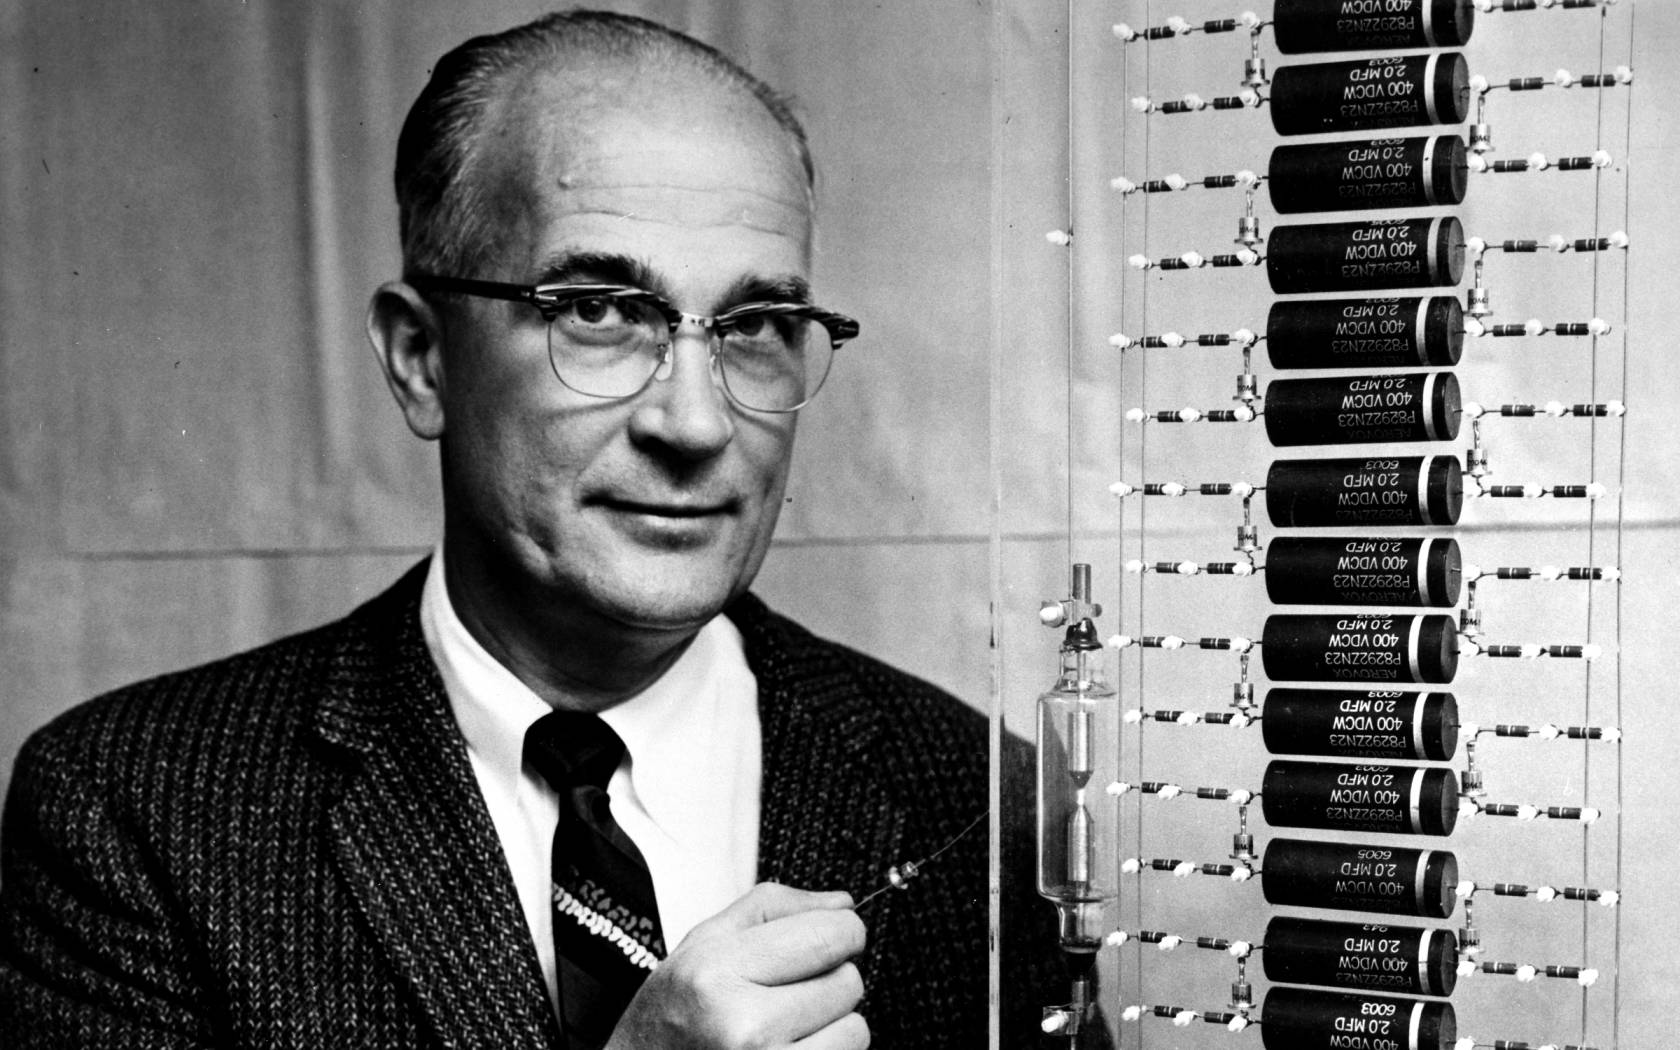
\includegraphics[height=0.65\textheight]{../../assets/William-Shockley.jpg} \\
                \vspace{0.2cm}
                \textbf{William Shockley} \\
                \small (1910 -- 1989)
            \end{center}
        \end{column}
        \begin{column}{0.6\textwidth}
            \vspace{0.5cm}
            \Large \textbf{El Teórico Formidable}
            
            \vspace{0.4cm}
            \normalsize
            Físico brillante, ambicioso y poseedor de un ego gigantesco. Formó el equipo para crear el amplificador de estado sólido, convencido de que sería su nombre el que pasaría a la historia.
            
            \vspace{0.4cm}
            Sin embargo, sus primeros diseños teóricos del transistor de efecto de campo fracasaron repetidamente en el laboratorio.
        \end{column}
    \end{columns}
\end{frame}

\begin{frame}{Los Subordinados}
    \begin{columns}
        \begin{column}{0.4\textwidth}
            \begin{center}
                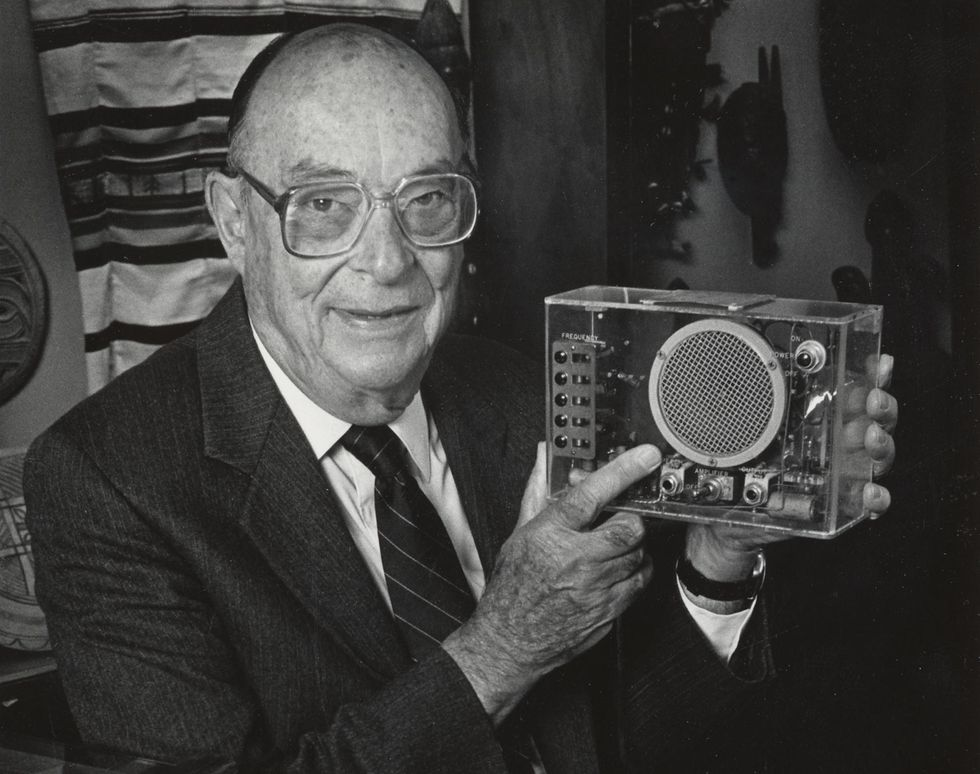
\includegraphics[height=0.65\textheight]{../../assets/John-Bardeen.jpg} \\
                \vspace{0.2cm}
                \textbf{John Bardeen} \\
                \small (1908 -- 1991)
            \end{center}
        \end{column}
        \begin{column}{0.6\textwidth}
            \vspace{0.5cm}
            \Large \textbf{El Genio Silencioso}
            
            \vspace{0.4cm}
            \normalsize
            Uno de los físicos teóricos más grandes de la historia (el único en ganar dos Premios Nobel de Física). Él entendió que los electrones quedaban atrapados en la \textit{superficie} del semiconductor.
        \end{column}
    \end{columns}
\end{frame}

\begin{frame}{El Ingeniero Experimental}
    \begin{columns}
        \begin{column}{0.4\textwidth}
            \begin{center}
                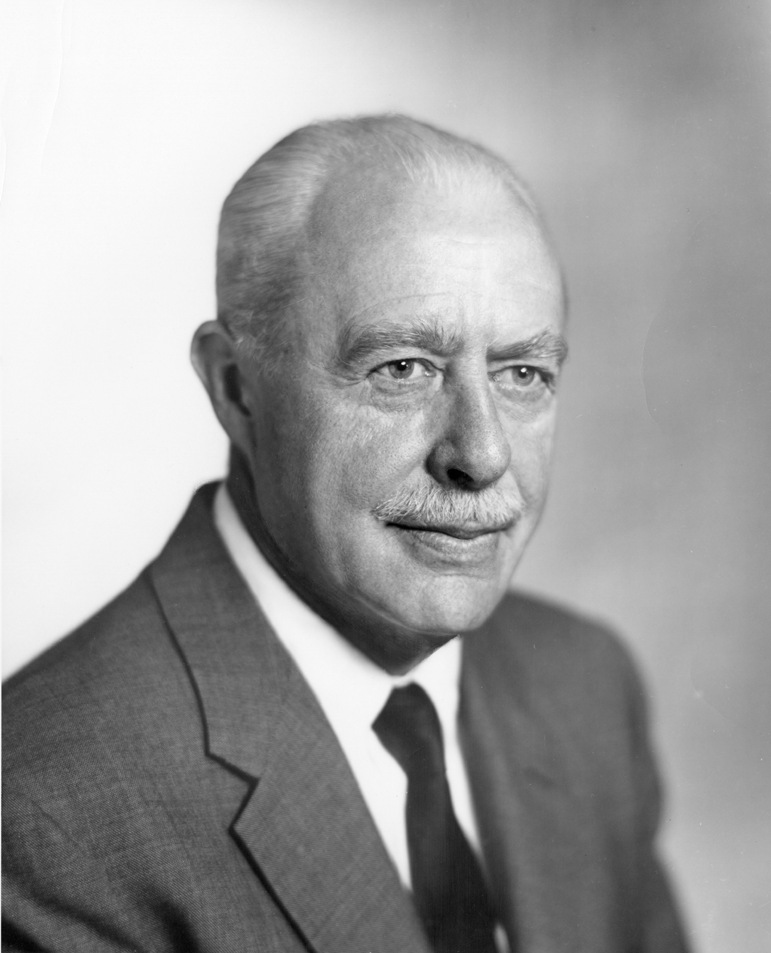
\includegraphics[height=0.65\textheight]{../../assets/Walter-Brattain.jpg} \\
                \vspace{0.2cm}
                \textbf{Walter Brattain} \\
                \small (1902 -- 1987)
            \end{center}
        \end{column}
        \begin{column}{0.6\textwidth}
            \vspace{0.5cm}
            \Large \textbf{Las Manos en la Materia}
            
            \vspace{0.4cm}
            \normalsize
            Mientras Shockley se frustraba y se alejaba del proyecto diario, Bardeen y Brattain formaron una alianza inquebrantable. Bardeen proveía las matemáticas; Brattain construía los dispositivos con oro y plástico a nivel microscópico.
        \end{column}
    \end{columns}
\end{frame}

\begin{frame}{El "Mes Mágico" y la Traición}
    \vspace{0.4cm}
    \Large \textbf{Diciembre de 1947}
    
    \vspace{0.6cm}
    \normalsize
    Trabajando a espaldas de Shockley, Bardeen y Brattain lograron aislar el problema y construyeron el \alert{\textbf{Transistor de Contacto Puntual}}. El dispositivo funcionaba a la perfección: amplificaba la señal sin tubos de vacío.
    
    \vspace{0.4cm}
    Cuando los abogados de patentes revisaron el invento, excluyeron el nombre de William Shockley, pues el principio físico usado no era el que él había propuesto inicialmente.
\end{frame}

\begin{frame}{La Venganza Teórica}
    \vspace{0.4cm}
    \Large \textbf{El Motor del Ego}
    
    \vspace{0.6cm}
    \normalsize
    Shockley, consumido por la furia de quedar fuera de la patente, se encerró en una habitación de hotel en Chicago. 
    
    \vspace{0.4cm}
    Impulsado por pura rabia para demostrar su superioridad intelectual frente a sus subordinados, desarrolló durante semanas y sobre el papel toda la teoría de las uniones PN que acabamos de ver.
    
    \vspace{0.4cm}
    Ahí inventó el \alert{\textbf{Transistor de Unión Bipolar}}, un diseño inmensamente superior que cambiaría el curso de la historia tecnológica para siempre.
\end{frame}

\begin{frame}{Hacia la Arquitectura Moderna}
    \vspace{0.8cm}
    \begin{center}
        \huge \textit{``Dominamos la termodinámica para imponer la lógica.''}
    \end{center}
    
    \vspace{0.8cm}
    \normalsize
    Toda la computación moderna, la inteligencia artificial, el software... todo existe gracias a que resolvimos físicamente cómo evitar que el calor mezcle los ceros y los unos.
    
    \vspace{0.6cm}
    \textbf{Próxima Sesión (Sesión 8):} Usaremos transistores (CMOS) para construir físicamente la compuerta NAND, la semilla del universo de Boole.
\end{frame}

\end{document}
